\documentclass[12pt]{article}

\usepackage{bm,graphicx, amssymb, amsmath}
\usepackage[margin=1 in]{geometry}
\usepackage{mathtools}
\usepackage{epstopdf}
\usepackage{enumitem}
\usepackage{color}

\newcommand{\ds}{\displaystyle}
\newcommand{\B}[1]{{\bm #1}}
\newcommand{\U}[1]{{\hat{\bm #1}}}
\newcommand{\T}{^{\mbox{\tiny T}}}

%\thispagestyle{empty}

\begin{document}

\newif\ifsolution    % Declaration, defaults to false

%% Comment out this line to hide solutions
% \solutiontrue
     
\begin{center}{\bf AERO-222: Introduction to Aerospace Computation, Spring 2023\\ Homework \#1, Due Date: Thursday, February 9, 2023} \vspace{0.5cm}

\textbf{\underline{Show all work and justify your answers!}} \vspace{0.5cm}
\end{center}

{\Large \textbf{Instructions}}

\begin{itemize}
	\item \textit{This homework contains both handwritten and coding problems and shall be submitted according to the following guidelines.}
	\item \textit{Hardcopy:}
	\begin{itemize}
	    \item \textit{Due on CANVAS at 11:59 PM on the day of the deadline.}
	    \item \textit{Shall include screenshots of any hand-written work.}
	    \item \textit{For coding problems, the hardcopy shall include any relevant derivations and emphasize the final results (i.e. boxed, highlighted, etc.).}
	    \item \textit{Shall be submitted as a single file according to the provided template with the following naming scheme:} ``LastnameHW\#.pdf"
	    \item \textit{If preferable, you can put all of your work into a single Jupyter notebook (.ipynb) with photos of your hand-written work as well. Markdown allows for images. }
	\end{itemize}
	\item \textit{Coding Submission:}
	\begin{itemize}
	    \item \textit{Due on CANVAS at 11:59 PM on the day of the deadline.}
	    \item \textit{Shall be submitted as a single file according to the provided template with the following naming scheme:} ``LastnameHW\#.py" or ``LastNameHW\#.ipynb".
	    \item \textit{The script shall print out all outputs asked for in the problem}.
	\end{itemize}
    \item \textit{Late submissions will be accepted with a 10 point deduction per day late.}
\end{itemize}
\hrulefill

\begin{description}
\item[1. Root-finding Algorithms \color{red} (Coding Problem) \color{black} (15 pts)]
Calculate the roots (to an absolute error $\varepsilon_x < 1e-08$) of
    \begin{equation*}
        f (x) = 3x^{2}\sin{x} - x\cos{x} + 4 = 0
    \end{equation*}
Use the following 3 methods:
    \begin{itemize}
   	\item Bisection method
   	\item Secant method
   	\item Regula-Falsi method
    \end{itemize}

    These methods require a set of starting points/bounds. Use $x_1 = -2$ and $x_2 = +2$, which will meet the initial requirements for all 3 methods. For each method, calculate and plot $f(x_{n})$ as a function of the iteration number $n$. Which method converges within the given tolerance in the fewest iterations?
    
    \color{red}
    \ifsolution
    {\bf Solution}:\\ The Secant Method converges the fastest.
    % Try and run the code. There is a chance they changed the code for each figure, but it should generate a correct solution.
    
    \begin{figure}[h!]
    	\centering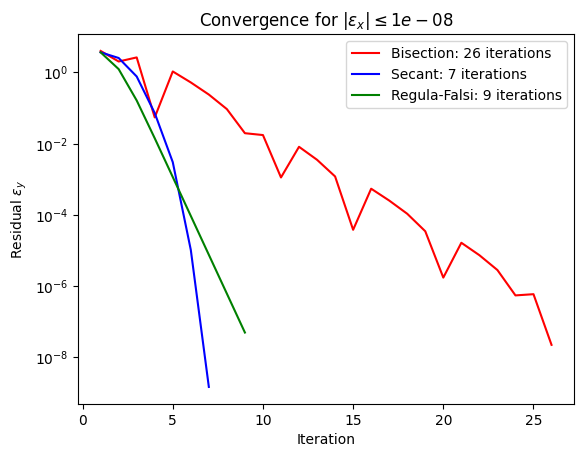
\includegraphics[width=4.5in]{HW1Fig1.png}
    	\caption{The solution should look very similar to this, all methods should converge to zero}
    	\label{fig:RootFindingAlgorithms}
    \end{figure}
    \fi
    \color{black}

\item[2. Round-off Error \color{red} (Coding Problem) \color{black} (10 pts)] Write a script to:
\begin{enumerate}[label=\textbf{(\alph*)}]
\item Evaluate the cubic polynomial, $f (x)$, at $x = 1.32$, using default machine precision and again using only three significant digits at each arithmetic operation. Calculate the absolute and relative error of the final result:
    \begin{equation*}
        f (x) = 3.15 \, x^3 - 2.11 \, x^2 - 4.01 \, x + 10.33
    \end{equation*}
    \item Repeat part (a) but do it with \emph{nested multiplication}. Compare errors. Which takes fewer operations? The nested form is:
    \begin{equation*}
        f (x) = [(3.15 \, x - 2.11) \, x - 4.01] \, x + 10.33
    \end{equation*}
    \end{enumerate}
    
    \color{red}
    \ifsolution
    {\bf Solution}:\\
    \begin{enumerate}[label=\textbf{(\alph*)}]
    \item With default machine precision:
    \begin{equation*}
        3.15 \times 1.32^3 - 2.11 \times 1.32^2 - 4.01 \times 1.32 + 10.33 = 8.82120625
    \end{equation*}
    With rounding to 3 significant digits in between operations (powers are treated as 1 operation):
    \begin{equation*}
    \begin{split}
     3.15 \times 1.32^3 + 2.11 \times 1.32^2 - 4.01 \times 1.32 + 10.33 &= 8.822    \\
    \text{Absolute Error} &= 7.9375 \times10^{-4} \\
    \text{Relative Error} &= 8.9982 \times10^{-5}	\\
    \text{Number of Steps} &= 9
    \end{split}
    \end{equation*}
    \item With default machine precision:
        \begin{equation*}
            [(3.15 \, x - 2.11) \, x - 4.01] \, x + 10.33 = 8.82120625
        \end{equation*}
        With rounding to 3 significant digits in between operations:
        \begin{equation*}
        \begin{split}
        [(3.15 \, x - 2.11) \, x - 4.01] \, x + 10.33 &= 8.822 \\
    \text{Absolute Error} &= 7.9375 \times10^{-4} \\
    \text{Relative Error} &= 8.9982 \times10^{-5} \\
    \text{Number of Steps} &= 6
    \end{split}
    \end{equation*}
    \end{enumerate}
    In this case, the errors are the same because both results round to the same value for 3 significant digits.
    The first approach is in general more accurate but requires more operations. If any very small values show different results (smaller than $10^{-10}$), its due to machine/python round-off errors.
    \fi
    \color{black}
    
\item[3. Truncation Error \color{red} (Coding Problem) \color{black} (20 pts)] Evaluate $f (x) = e^{-5}$ to four digits of precision (chopping) using the following two approaches:
    \begin{enumerate}[label=\textbf{(\alph*)}]
    \item $e^{-5} = \ds\sum^7_{k = 0} \dfrac{(-5)^k}{k!} = \ds\sum^7_{k = 0} \dfrac{(-1)^k 5^k}{k!}$
    \item $e^{-5} = \dfrac{1}{e^5} \approx \dfrac{1}{\ds\sum^7_{k = 0} \dfrac{(5)^k}{k!}}$
    \end{enumerate}
    Note that the true value to four digits of precision is $1.8316 \times 10^{-2}$. Which formula gives more accurate results and why? Plot the error of each approach as a function of iteration number.

    \color{red}
    \ifsolution
    {\bf Solution}:
    \begin{enumerate}[label=\textbf{(\alph*)}]
    \item $1-5+12.5-20.83+26.04-26.04+21.70-15.50+9.69-5.38+2.69 = 8.6404 \times 10^{-1}$ 
    \item $1/(1+5+12.5+20.83+26.04+26.04+21.70+15.50+9.69+5.38+2.69)  = 6.8315 \times 10^{-3}$
    \end{enumerate}
    The actual value to 4 digits of precision is $6.7379 \times 10^{-3}$. The second method is more accurate because it does not oscillate about the value, but instead always stays smaller than 1 and larger than 0. Thus, the truncation error of the     \begin{figure}[h!]
	\centering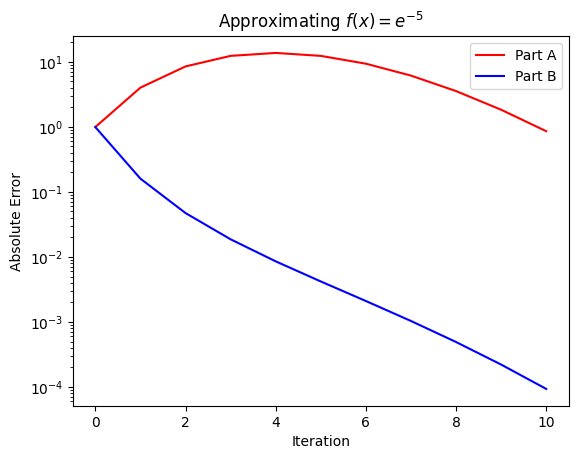
\includegraphics[width=4.5in]{HW1Fig2.png}
	\caption{Method 2 is more accurate}
	\label{fig:truncationError}
\end{figure}second method is lower for the same number of steps.
    
    
    \fi
    \color{black}
    
\item[4. Taylor Series (15 pts)] Expand the function, $f (x) = x^4 + \sin{x}$, by Taylor series up to degree 3 for the following cases:
    \begin{enumerate}[label=\textbf{(\alph*)}]
	\item centered at $x_0 = 4$ and evaluated at $x_1 = x_0 + 0.2$;
	\item centered at $x_0 = 3$ and evaluated at $x_1 = x_0 - 0.7$.
    \end{enumerate}

    \color{red}
    \ifsolution
    {\bf Solution}:\\
    First write the general form of the Taylor polynomial for clarity:
    \begin{equation*}
        f(x) \approx f(x_0) + f'(x_0) (x - x_0)+ \dfrac{f'' (x_0) (x - x_0)^2}{2!}+ \dfrac{f''' (x_0) (x - x_0)^3}{3!}
    \end{equation*}
    Then, insert the given equation:
    \begin{equation*}
        f(x) \approx x_0^4+\sin{x_0} + (4x_0^3+\cos{x_0})(x-x_0)+ \dfrac{(12x_0^2-\sin{x_0})(x-x_0)^2}{2!}+ \dfrac{(24x_0-\cos{x_0} )(x-x_0)^3}{3!}
    \end{equation*}
    Insert given values:

    \item a. centered $x_0=4$ and evaluated $x_0 + 0.2 = 4.2$
    \begin{equation*}
        f(x) \approx 4^4+\sin{4} + (4(4)^3+\cos{4})(0.2)+ \dfrac{(12(4)^2-\sin{4})(0.2)^2}{2!}+ \dfrac{(24(4)-\cos{4})(0.2)^3}{3!}
    \end{equation*}
    \textbf{answer:} $310.296$

    \item b. centered $x_0=3$ and evaluated $x_0 - 0.7 =2.3$
    \begin{equation*}
        f(x) \approx 3^4+\sin{3} + (4(3)^3+\cos{3})(-0.7)+ \dfrac{(12(3)^2-\sin{3})(-0.7)^2}{2!}+ \dfrac{(24(3)-\cos{3})(-0.7)^3}{3!}
    \end{equation*}
    \textbf{answer:} $28.4869$
    \fi
    \color{black}

\item[5. Variables and Computer Precision (10 pts)]  Answer the following questions:
	\begin{enumerate}[label=\textbf{(\alph*)}]
		\item Which can store a larger number, a signed int or unsigned int?
		\item Which uses more memory, a float or double? Which is more precise?
		\item If I'm trying to establish if two integers are equal, what's the easiest way to compare their values in code? Write the statement that would achieve this?
		\item If I'm trying to establish if two real numbers (double or float) are equal, what's the ``correct" way to compare their values in code? Write the statement that would achieve this.
		\item What is Python default machine precision?
	\end{enumerate}
	
	\color{red}
	\ifsolution
	{\bf Solution}:
    \begin{enumerate}[label=\textbf{(\alph*)}]
		\item unsigned int
		\item double, double
		\item a == b
		\item $|a - b| < \epsilon$
		\item Double (64 bits or I will also accept 53 bit if they are talking about the mantissa), 9223372036854775807, (\verb"sys.maxsize") 1.7976931348623157e+308 (\verb"sys.float_info.max") [10e+4931 with numpy]
	\end{enumerate}
	\fi
	\color{black}

\item[6. Base Conversion (10 pts)] Show all steps:
\begin{enumerate}[label=\textbf{(\alph*)}]
		\item Convert 1482 from decimal to binary.
		\item Convert 0.1 from decimal to binary using 1 byte (8 bits).
		\item Does adding zeros to the back (ones side) of a base 10 integer change the value? What about a base 2 (binary) integer?
		\item Now consider the value to be a decimal. Does anything change?
	\end{enumerate}
	
	\color{red}
	\ifsolution
	{\bf Solution}:
    \begin{enumerate}[label=\textbf{(\alph*)}]
		\item 10111001010
		\item 0.00011001
		\item Yes, yes
		\item No (the number is unchanged)
	\end{enumerate}
	\fi
	\color{black}

\item[7. Error Propagation (20 pts)] Consider the following two statements,
\begin{align*}
    z &= 2 x - y + \sin(x y^2) \\
    w &= e^z - 2 (z^2 - 1)
\end{align*}
with mean values $\mu_x = 3$ and $\mu_y = 2$, and standard deviations $\sigma_x = 0.02$ and $\sigma_y = 0.01$. Estimate the following parameters using four significant digits: 
	\begin{enumerate}[label=\textbf{(\alph*)}]
	\item $\mu_w$
	\item $\sigma_w$
	\end{enumerate}

    \color{red}
    \ifsolution
    {\bf Solution}:\\
    \begin{enumerate}[label=\textbf{(\alph*)}]
    
    \item $\mu_z = 2 \mu_x - \mu_y + \sin(\mu_x \, \mu_y^2) = 3.4634\\
    \mu_w = e^{\mu_z} - 2 (\mu_z^2 - 1) = 9.9355$
    
    \item Partial derivatives:
    \begin{align*}
       \frac{\partial z}{\partial x}\Bigr\rvert_{\mu_x,\mu_y} &= 2 + \mu_y^2 \, \cos(\mu_x \mu_y^2) = 5.375 \\
       \frac{\partial z}{\partial y}\Bigr\rvert_{\mu_x,\mu_y} &= -1 + 2\mu_x \mu_y \, \cos(\mu_x \mu_y^2) = 9.126 \\
       \frac{\partial w}{\partial z}\Bigr\rvert_{\mu_z} &= e^{\mu_z} - 4z = 18.072;
    \end{align*}
    Then, the standard deviation of $z$ becomes,
        \begin{equation*}
       \sigma_z = \sqrt{\frac{\partial z}{\partial x}\Bigr\rvert_{\mu_x,\mu_y}^2 \, \sigma_x^2 + \frac{\partial z}{\partial y}\Bigr\rvert_{\mu_x,\mu_y}^2 \, \sigma_y^2} = 0.14102
    \end{equation*}
    and the standard deviation of $w$ is,
        \begin{equation*}
       \sigma_w = \sqrt{\frac{\partial w}{\partial z}\Bigr\rvert_{\mu_z}^2 \, \sigma_z^2} = 2.549
    \end{equation*}
    
    \end{enumerate}
    \fi
    \color{black}
\end{description}
\end{document}